\documentclass[12pt,norsk,a4paper]{article}
\usepackage{graphicx}
\usepackage{verbatim}
\usepackage{hyperref}
\usepackage{float}
\usepackage{ulem}
\usepackage{multirow}
\newcommand*\xor{\mathbin{\oplus}}
\usepackage[utf8]{inputenc}
\usepackage[norsk]{babel}

\begin {document}
\title{Dig Tek - Øving 5}
\author {Arve Nygård}

\maketitle

\clearpage

\section{Oppgave 1}

\subsection{Deloppgave a}

\begin{figure}[H]
\begin{center}
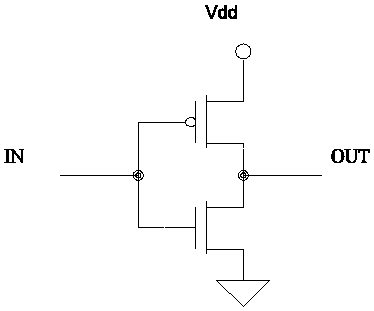
\includegraphics[scale=0.5]{inverter.png}
\caption{Inverter}
\end{center}
\label{fig:ideellgraf}
\end{figure}


Når $V_{in}$ er høy, vil P-MOS transistoren blokkere strømen fra $5V$, mens N-MOS transistoren vil slippe strøm igjennom fra jord, til $V_{out}$
Når $V_{in}$ er lav, vil det motsatte skje; signalet fra $5V$ slippes gjennom til $V_{out}$, mens signalet fra jord blokkeres.


\subsection{Deloppgave b}
\begin{equation}
P = \frac{1}{2} \alpha f C V_{dd}^2
\end{equation}

$\alpha$: aktivitetsfaktor, $f$: klokkefrekvens \\
\\
Motstanden i N-MOS og P-MOS vil gi et effektforbruk ved overgang fra 0 til 1, og omvendt.

\section{Oppgave 2}
\subsection{a}
\begin{table}[H]
\begin{center}
    \begin{tabular}{ |c|c|c| }
    \hline
    \multirow{2}{*}{Desimaltall} & Binærtall & Binærtall\\
    & (Sign-magnitude) & (2's komplement) \\ \hline
    7   & 0111          &  0111\\ \hline
    6   & 0110          &  0110\\ \hline
    5   & 0101          &  0101\\ \hline
    4   & 0100          &  0100\\ \hline
    3   & 0011          &  0011\\ \hline
    2   & 0010          &  0010\\ \hline
    1   & 0001          &  0001\\ \hline
    0   & 0000 / 1000   &  0000\\ \hline
    -1  & 1001          &  1111\\ \hline
    -2  & 1010          &  1110\\ \hline
    -3  & 1011          &  1101\\ \hline
    -4  & 1100          &  1100\\ \hline
    -5  & 1101          &  1011\\ \hline
    -6  & 1110          &  1010\\ \hline
    -7  & 1111          &  1001\\ \hline
    -8  & -             &  1000\\ \hline
    
    \end{tabular}
    \end{center}
    \caption{Komplement tall aritmetikk. Merk at kun 15 distinkte verdier kan representeres med Sign-magnitude, mens 16 verdier kan representeres med 2's komplement. Grunnen til dette er at 0 har to forskjellige representasjoner i sign-magnitude.}
\end{table}

\clearpage
\subsection{b}
$A = 6_{10} = 0110$ \hspace{0.5cm} , \hspace{0.5cm}  $-A = -6_{10} = 1010$\\
$B = 5_{10} = 0101$ \hspace{0.5cm} , \hspace{0.5cm} $-B = -5_{10} = 0111$\\
\begin{table}[H]
    \begin{tabular}{cr}
    \multirow{3}{*}{$A-B = A+(-B)$: } & $  0110$\\
                                     & $+\uline{1011}$\\
                                     & $=\uuline{0001}$
    \end{tabular}
\end{table}
$0001$ = $1_{10}$. OK!

\begin{table}[H]
    \begin{tabular}{cr}
    \multirow{3}{*}{$B-A = B+(-A)$: } & $  0101$\\
                                     & $+ \uline{1010}$\\
                                     & $= \uuline{1111}$
    \end{tabular}
\end{table}
1111 = $-1_{10}$. OK!

\subsection{c}
Hvis $MSB$ i begge summandene er like, men $MSB$ i resultatet er forskjellig fra disse to, har vi overflow.
\begin{table}[H]
    \begin{center}
    \begin{tabular}{|r|}
    \hline
    $ \textbf{A}xxxx$\\
    $+\uline{\textbf{A}xxxx}$\\
    $=\uuline{\overline{\textbf{A}}xxxx}$\\
    \hline
    \end{tabular}
    \end{center}
    \caption{Eksempel på overflow.}
\end{table}


\subsection{d}
$C = -8_{10} = 1000_{2's kompl.}$ \hspace{1cm}, \hspace{1cm} $D=-3_{10} = 1101_{2's kompl.}$

\begin{table}[H]
    \begin{tabular}{cr}
    \multirow{3}{*}{$B-A = B+(-A)$: } & $  1000$\\
                                     & $+ \uline{1101}$\\
                                     & $= \uuline{0101}$
    \end{tabular}
    \caption{MSB til $C$ og $D$ er forskjellig fra MSB til svaret. Vi får overflow.}
\end{table}

\subsection{e}

$10110_{2}$ utvidet til 7 bits notasjon: Vi kopierer MSB, setter den inn på venstre siden, og får $1110110_2$. \\
Svaralternativ e3 er derfor korrekt. 

\clearpage
\section{Oppgave 3}
\subsection{a}
$A = -11_{10} = 10101_2$ \hspace{1cm},\hspace{1cm} $B = -13_{10} = 10011_2$

$A*B:$
    
\begin{table}[H]
\begin{center}
    \begin{tabular}{ r|c|c | l }
    \hline 
     & A & B & kommentar\\
    \hline
    1 & 10101 & 10011 &  \\ 
    \hline
    1 & 10101 & 00000 & \textit{1.Partielle Produkt}\\ 
    1 & 11010 & 10000 & \textit{Shift Right}\\
    1 & 10101 & 00000 & \textit{2.PP}\\
    \hline
    1 & 01111 & 10000 & \textit{Sum}\\
    1 & 10111 & 11000 & \textit{SR}\\
    1 & 11011 & 11100 & \textit{3.PP = 0, SR}\\
    1 & 11101 & 11110 & \textit{4.PP = 0, SR}\\
    1 & 10101 & 00000 & \textit{5.PP, trekk fra siden vi brukte MSB.}\\
    \hline
    0 & 01000 & 11110 & \textit{Sum,SR}\\
      & \textbf{00100} & \textbf{01111} & \textit{Resultat}\\
      \hline \hline
    \end{tabular}
    \end{center}
    \caption{Binær Multiplikasjon}
\end{table}


\subsection{b}

$160_{10}:7_{10}$ = $10100000_{2} : 111_{2}$

\begin{verbatim}
 10100000:111 = 10110
- 111
  0110
-  000
  01100
-   111
  001010
-    111
  0000110
-     000
      110  <-- Rest   
\end{verbatim}

Svar: \uuline{10110 + 110 }

\clearpage
\section{Oppgave 4}
\subsection{a)}
\subsubsection{1)}

$1101011_{Gray} = \uuline{1001101_{Bin}}$\\
$B_{i-1}  G_i  B_i$\\
$0 \xor 1 = 1$\\
$1 \xor 1 = 0$\\
$0 \xor 0 = 0$\\
$0 \xor 1 = 1$\\
$1 \xor 0 = 1$\\
$1 \xor 1 = 0$\\
$0 \xor 1 = 1$\\



\subsubsection{2)}
$1001101_{Gray} = \uuline{1110110_{Bin}}$\\
$B_{i-1}  G_i  B_i$\\
$ 0 \xor 1 = 1 $\\
$ 1 \xor 0 = 1 $\\
$ 1 \xor 0 = 1 $\\
$ 1 \xor 1 = 0 $\\
$ 0 \xor 1 = 1 $\\
$ 1 \xor 0 = 1 $\\
$ 1 \xor 1 = 0 $\\


\clearpage
\subsection{b)}
\subsubsection{1)}
$0111111{Bin} = \uuline{0100000_{Grey}}$
  
$ 0 \xor 0 = 0 $\\
$ 0 \xor 1 = 1 $\\
$ 1 \xor 1 = 0 $\\
$ 1 \xor 1 = 0 $\\
$ 1 \xor 1 = 0 $\\
$ 1 \xor 1 = 0 $\\
$ 1 \xor 1 = 0 $\\

\subsubsection{2)}
$1000000{Bin} = \uuline{1100000_{Grey}}$
  
$ 0 \xor 1 = 1 $\\
$ 1 \xor 0 = 1 $\\
$ 0 \xor 0 = 0 $\\
$ 0 \xor 0 = 0 $\\
$ 0 \xor 0 = 0 $\\
$ 0 \xor 0 = 0 $\\
$ 0 \xor 0 = 0 $\\
\clearpage
\section{Oppgave 5}
\subsection{a)}
$Q_1$ tilhører D-vippen (flip-flop)
$Q_2$ tilhører D-låsen.
\subsection{b)}
$T_{Oppsett}$ er tiden der innsignalet må være uendret før en flanke for at endringen skal bli registrert av kretsen. \\
$T_{Hold}$ er tiden der inngangssignalet må være uendret etter en flanke for at endringen skal bli registrert av kretsen.
\end{document}